\section{Estruturas Propostas}

\subsection{Dense Advanced Myers List} \label{subsec:dense_list}

A Dense Advanced trata-se de uma variação da Advanced Myers List criada por Peters \cite{peters2025}, mas em vez de dividir um nó com dois a quatro
apontadores, em um a três células, cada uma com dois apontadores. Decidimos representar cada nó com uma única célula, com o seu respetivo número de 
apontadores:

\begin{lstlisting} [style=ocaml_light, caption={Tipos de células}, captionpos=b, float=h]
type 'a add_points = 
    | Normal 
    | Skip of 'a cell 
    | Leaf of 'a cell * 'a cell
and 'a cell = { next : 'a cell; jump : 'a cell; length : int; 
    value : 'a; rhd : int; red : int; more : 'a add_points }
\end{lstlisting}

Isto tornou a implementação da estrutura mais fácil e por consequência, determinar o algoritmo para a operação \textit{cons} foi mais simples.
Outros benefícios desta alteração foram: Um número de travessias de apontadores menor; Encontraram-se novas otimizações que não foram ponderadas
na implementação original; E obteve-se um \textit{lookup} mais rápido.

No entanto, um defeito desta estrutura em relação à original, é que esta gasta mais memória, já que cada célula contém mais apontadores.

O caso uso mais apropriado para esta estrutura seria um ambiente onde a travessia de apontadores seria muito custosa, tal como referido para a 
lista original: «Thus, advanced Myers lists may not be appropriate for in-memory lists, but they may be useful for applications where the cost 
of pointer traversals is high relative to other computations, such as when pointer traversals involve network access.» (Peters et al., 2025, p. 13)


\begin{figure}[H]
    \centering
    
    \subfloat[Formato de lista]{
        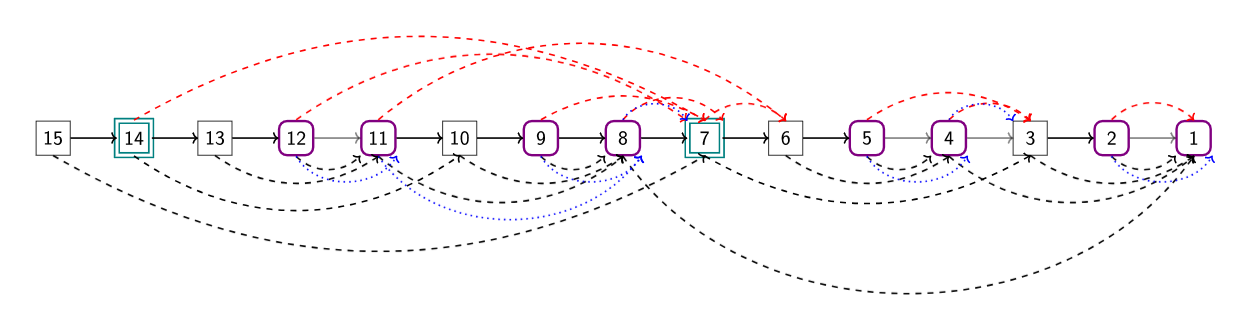
\includegraphics[width=0.48\linewidth]{Imagens/Dense-Lista}
    }
    \hfill
    \subfloat[Formato de árvore]{
        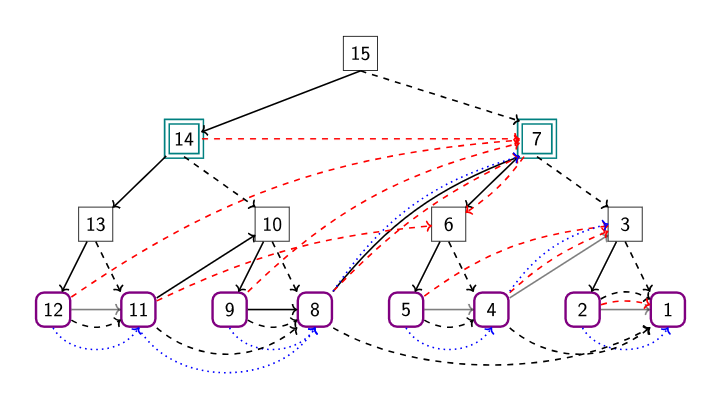
\includegraphics[width=0.48\linewidth]{Imagens/Dense-Arvore}
    }
    \caption{Representação da Dense Advanced Myers List}
    \label{fig:Dense}
\end{figure}


\subsubsection{\textit{Cons}}

Na Dense Advanced Myers List, o \textit{cons} difere das restantes variantes, uma vez que este não apresenta um \textit{cons} em tempo constante. 
A inserção de um novo elemento exige sempre o cálculo do RED e do RHD, além da atribuição dos apontadores \texttt{next} e \texttt{jump}. 
\\

O algoritmo determina o tipo de nó a ser criado com base na altura lógica e avaliando em relação ao $\sigma$. O motivo desta estrutura não 
apresentar um \textit{cons} em tempo constante deve-se a criação de novas células \textit{skip} (\texttt{Skip}) e folha (\texttt{Leaf}), estas células apresentam apontadores adicionais: \texttt{inc} e 
\texttt{uncle}. Que para receberem o valor apropriado é necessário atravessar a própria estrutura da lista à procura das células apropriadas com base 
nos valores do RED e RHD.


\subsubsection{\textit{Lookup}}

O algoritmo de \textit{lookup} na Dense Myers List é como uma busca hierárquica. Quando solicitamos o \textit{lookup} por um elemento em uma posição específica, 
o algoritmo primeiro calcula a distância que precisa para chegar ao alvo e avalia o tipo de nó atual, que pode ser uma célula do tipo normal, 
\textit{skip} ou folha. Se o destino estiver longe, o algoritmo usa os apontadores adicionais, \texttt{uncle} e \texttt{inc}. À medida que o algoritmo se aproxima do local 
desejado e a distância diminui, ele deixa de usar esses atalhos grandes e entra em uma etapa de descida. Nessa etapa final, ele faz saltos menores, 
\texttt{next} ou \texttt{jump}, até chegar com exatidão ao elemento procurado.


\subsection{Improved Applicative Random-Access Stack with Sigma region} \label{subsec:iarass}

A Improved Applicative Random-Access Stack with Sigma region (IARASS) é uma variante da Improved Myers List que se beneficia da introdução do 
conceito de \textit{sigma layers}, introduzido por Peters \cite{peters2025} na Advanced Myers List. Assim, o objetivo da IARASS é utilizar este novo apontador
para aliviar o problema da descida dupla (\textit{double descent}) identificado no artigo original, sem perder a simplicidade estrutural existente na variante Improved.
Na secção dos Resultados, mostraremos ainda que esta estrutura, como é de esperado, apresenta um maior uso de memória que a Improved Myers List, 
no entanto apresenta um menor uso de memória quando comparada com a Advanced Myers List e apresentando um maior desempenho no número de travessias 
quando comparada com ambas as variantes.
\\

Ao contrário da Improved Myers List em que todas as células apresentam a mesma estrutura, contendo os campos \texttt{next}, \texttt{jump}, \texttt{length} e \texttt{value}, a IARASS 
distingue dois tipos de células:

\begin{lstlisting} [style=ocaml_light, caption={Tipos de células}, captionpos=b]
type 'a cell = 
  | Normal of {next:'a cell; jump:'a cell; length:int; value:'a; height:int }
  | Skip of {next:'a cell; jump:'a cell; length:int; value:'a; height:int; shortcut:'a cell }
\end{lstlisting}

Nesta variante, as células normais mantêm apenas os dois apontadores já existente na variante Improved Myers List mantendo toda a lógica já existente, 
enquanto as células \textit{skip} (células de salto) apresentam um terceiro apontador, denominado \texttt{shortcut}. A decisão de qual célula é criada é baseada na altura (\texttt{height}). 

\begin{figure}[H]
    \centering
    
    \subfloat[Formato de lista]{
        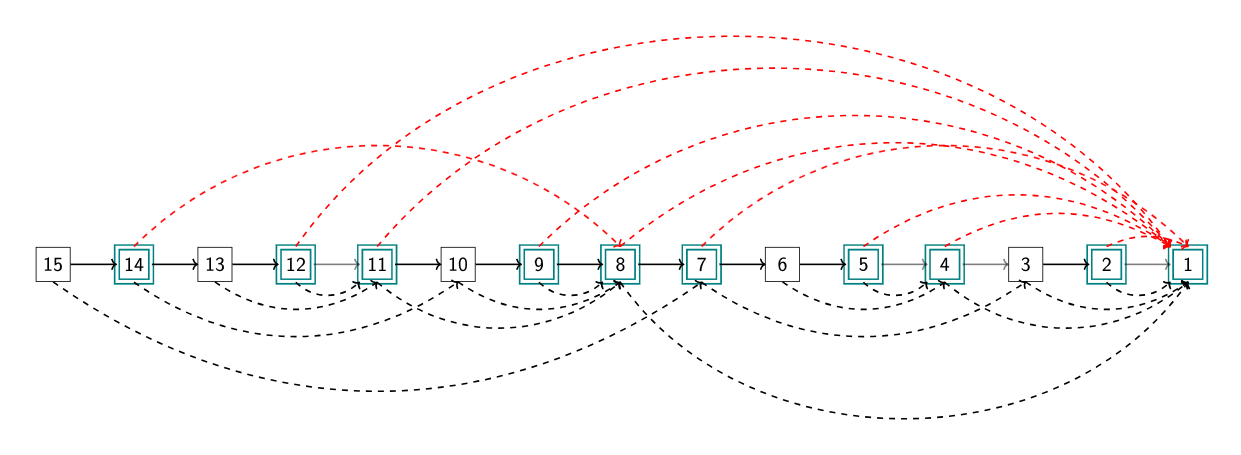
\includegraphics[width=0.48\linewidth]{Imagens/Iarass-Lista}
    }
    \hfill
    \subfloat[Formato de árvore]{
        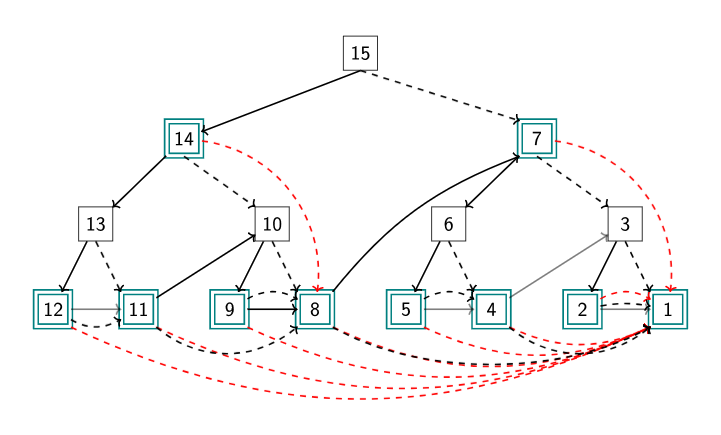
\includegraphics[width=0.4\linewidth]{Imagens/Iarass-Arvore.png}
    }
    \caption{Representação da IARASS}
    \label{fig:Iarass}
\end{figure}

\subsubsection{\textit{Cons}}

Durante a contrução de uma nova célula,
sempre que a altura é um divisor de $\sigma$, ou seja $\texttt{height} \bmod \sigma = 0$, a célula criada é do tipo \textit{skip} e nas restantes camadas serão do tipo normal. 
Ao contrário da Advanced Myers List, um $\sigma$ maior não indica uma melhor performance no \textit{lookup}, nesta estrutura a lógica é inversa, ou seja, quanto maior o $\sigma$ maior 
será o número de travessias, mas consequentemente usará menos memória.
\\

O novo apontador \texttt{shortcut} destas células \textit{skip} é a contribuição principal para resolver o problema da descida dupla e assume um comportamento diferente 
dependendo da posição da célula na árvore lógica: \textbf{(i)} quando a altura é diferente de 0, o \texttt{shortcut} aponta para a última célula da região que 
contém a célula acabada de ser criada. \textbf{(ii)} quando a altura é igual a 0, o \texttt{shortcut} aponta para \texttt{c.jump.jump.jump}, permitindo uma travessia horizontal 
mais rápida do que antes.  


\begin{comment}
A IARASS apresenta um \textit{cons} em tempo constante $\mathcal{O}(1)$ e apresenta um \textit{cons} muito semelhante a Improved Myers List, apenas diferenciando-se na ocasião dos nós 
\textit{skip}. Durante a inserção de um novo elemento, a altura lógica do novo nó a ser inserido é calculada, esta altura é utilizada para distinguir as 
células normais das células \textit{skip}. Sempre que a altura calculada for um divisor de $\sigma$, significa que a célula a ser criada é uma célula  \textit{skip}, caso 
contrário, a célula a ser criada é uma célula normal.

A atribuição do \texttt{shortcut} às células \textit{skip} difere dependendo da altura em que esta célula se encontra: \textbf{(i)} para alturas diferentes de 0, 
o \texttt{shortcut} aponta para o último elemento da região onde está inserida \textbf{(ii)} para alturas iguais a 0, o \texttt{shortcut} aponta para 3 saltos mais à frente, 
ou seja \texttt{get\_jump (get\_jump (get\_jump c))}.
\end{comment}

\subsubsection{\textit{Lookup}}

O algoritmo de \textit{lookup} na IARASS mantém-se idêntico à Improved Myers List nas células normais. Nas células \textit{skip}, o algoritmo verifica 
primeiro se é possível utilizar o \texttt{shortcut} para efetuar um salto maior, caso o \texttt{shortcut} ultrapasse a posição desejada, o algoritmo avalia o 
apontador \texttt{jump} e caso este também ultrapasse a posição desejada, optamos pela última opção de seguir pelo apontador \texttt{next}. 
